\subsubsection{Modelo conceptual}

\subsubsection{Diagrama}
\begin{figure}[p!hbt]
		\centering
		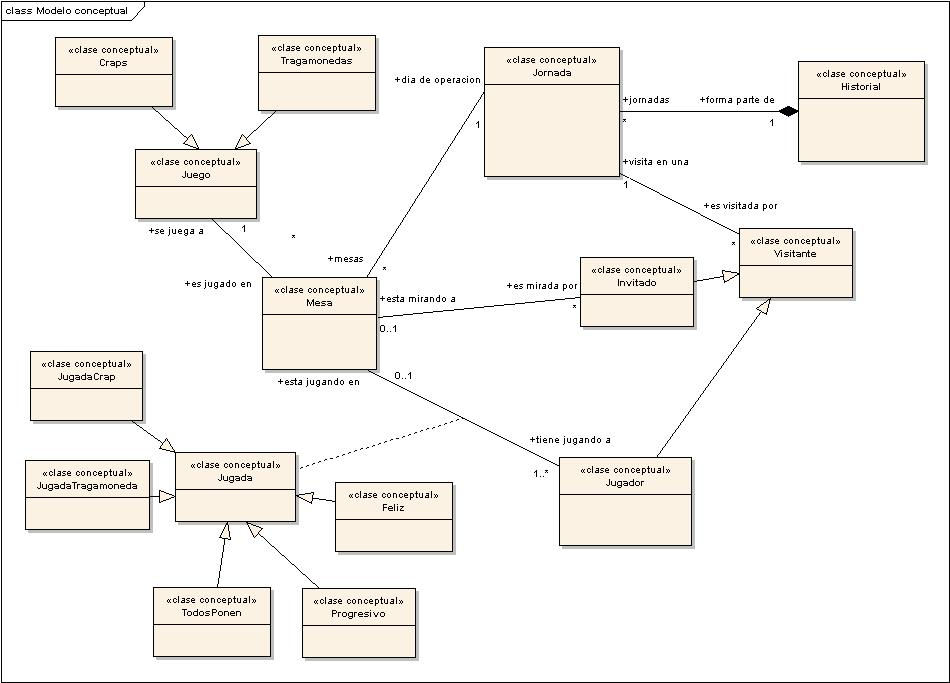
\includegraphics[angle=90, width=1.0\textwidth]{../img/ModeloConceptual.png}
		\caption{Diagrama de clases conceptuales}
\end{figure}
% \imagen{../img/ModeloConceptual.png}{Diagrama de clases conceptuales}{0.5}

\begin{itemize}
 \item \textit{ Solo hay una jugada feliz como m'aximo \\}
  \textbf{context} Jugada 
  \\ \textbf{inv:} 
  Jugada.allInstances()$\rightarrow$select(tipo = TipoJugada::feliz)$\rightarrow$size() $\leq$ 1)


\item \textit{ Para cada mesa de Craps hay exactamente un tirador \\}
\textbf{context}  MesaDeCraps \\ \textbf{inv:} 
  self.Jugada$\rightarrow$select(j $|$ j.oclAsType(JugadaCrap).tirador = true)$\rightarrow$size() = 1)


\item \textit{En las mesas de Craps s'olo se realizan apuestas de tipo Crap} 

\textbf{context}  MesaDeCraps \\ \textbf{inv:} 
  self.Jugada$\rightarrow$forAll(j $|$ j.oclIsTypeOf(JugadaCrap))


\item \textit{En las mesas de Tragamonedas s'olo se realizan apuestas de tipo Tragamoneda}

\textbf{context}  MesaDeTragamonedas \\ \textbf{inv:} 
  self.Jugada$\rightarrow$forAll(j $|$ j.oclIsTypeOf(JugadaTragamoneda))

\item \textit{Los jugadores comunes no tienen saldo negativo}

\textbf{context}  JugadorComun \\ \textbf{inv:} 
  self.saldo $\geq$ 0

\item \textit{ No hay jugadores con el mismo dni}

\textbf{context}  Jugador \\ \textbf{inv:} 
  Jugador.allInstances()$\rightarrow$forAll($j_{1}$, $j_{2}$ : Jugador $|$ $j_{1} < > j_{2}$ \textbf{implies} $j_{1}.dni < > j_{2}.dni$)


\item \textit{Los jugadores son comunes o vip}

\textbf{context}  Jugador \\ \textbf{inv:} 
  self.oclIsTypeOf(JugadorComun) or self.oclIsTypeOf(JugadorVip)


\item \textit{Las mesas son de tragamonedas o craps}

\textbf{context}  Mesa \\ \textbf{inv:} 
  self.oclIsTypeOf(MesaDeTragamonedas) or self.oclIsTypeOf(MesaDeCraps)


\item \textit{Las jugadas son de tragamonedas o craps}

\textbf{context}  Jugada \\ \textbf{inv:} 
  self.oclIsTypeOf(JugadaCrap) or self.oclIsTypeOf(JugadaTragamoneda)


\item\textit{ El tipo de jugada (normal, feliz o todosPonen) tiene que ser el mismo para las jugadas de una misma mesa}

\textbf{context}  Mesa \\ \textbf{inv:} 
  self.Jugada$\rightarrow$forAll($j_{1}$, $j_{2}$ : Jugada $|$ $j_{1}$.tipo = $j_{2}$.tipo)


\item\textit{ En una jugada Crap las apuestas en sitio a ganar de un jugador son a distintos n'umeros}

\textbf{context}  JugadaCrap \\ \textbf{inv:} 
  self.ApuestaEnSitioAGanar$\rightarrow$forAll( $a_{1}, a_{2}$ : ApuestaEnSitioAGanar $ | $ $ a_{1} <> a_{2} $  \textbf{implies} $ a_{1}.valor <> a_{2}.valor $ )


\item\textit{ En una jugada Crap las apuestas en sitio a perder de un jugador son a distintos n'umeros}

\textbf{context}  JugadaCrap \\ \textbf{inv:} 
  self.ApuestaEnSitioAPerder$\rightarrow$forAll($a_{1}$, $a_{2}$ : ApuestaEnSitioAPerder  $ | $ $a_{1} <> a_{2} $ \textbf{implies} $a_{1}$.valor $<>$ $a_{2}$.valor)

\end{itemize}
